\documentclass{article}
\usepackage[utf8]{inputenc}

\usepackage{graphicx}
\usepackage{listings}
\usepackage{color}
\usepackage[T1]{fontenc}
\usepackage{lmodern}
\usepackage{textcomp}
 
\definecolor{codegreen}{rgb}{0,0.6,0}
\definecolor{codegray}{rgb}{0.5,0.5,0.5}
\definecolor{codepurple}{rgb}{0.58,0,0.82}
\definecolor{backcolour}{rgb}{0.95,0.92,0.92}
 
\lstdefinestyle{pythonstyle}{
    language=Python,
    upquote=true,
    backgroundcolor=\color{backcolour},   
    commentstyle=\color{codegreen},
    keywordstyle=\color{magenta},
    numberstyle=\tiny\color{codegray},
    stringstyle=\color{codepurple},
    basicstyle=\footnotesize\ttfamily,
    basewidth={0.5em,0.5em},
    breakatwhitespace=false,         
    breaklines=true,                 
    captionpos=b,                    
    keepspaces=true,                 
    %numbers=left,                    
    %numbersep=5pt,                  
    showspaces=false,                
    showstringspaces=false,
    showtabs=false,                  
    tabsize=4
}

\lstdefinestyle{bashstyle}{
    language=bash,
    upquote=true,
    backgroundcolor=\color{backcolour},   
    commentstyle=\color{codegreen},
    basicstyle=\footnotesize\ttfamily,
    basewidth={0.5em,0.5em},
    breakatwhitespace=false,         
    breaklines=true,                 
    captionpos=b,                    
    keepspaces=true,                 
    %numbers=left,                    
    %numbersep=5pt,                  
    showspaces=false,                
    showstringspaces=false,
    showtabs=false,                  
    tabsize=4
}
 
\lstset{style=bashstyle}
 
\begin{document}

\title{Getting started with Auroraplot}
\date{}
\maketitle

\section{Minimum requirements}
Auroraplot has been tested on Fedora 24, Ubuntu 16.04 LTS, and Debian 8.
It should work on Apple OSX with minimal changes to the configuration steps.
Microsoft Windows is not currently supported.

Loading and manipulating large data sets requires significant amounts of RAM.
On systems with 8 GB frequent swapping to disk and slow-downs can occur,
especially when creating Quiet Day Curves. 16 GB or more is recommended.

\section{Installing Auroraplot}

Install the dependencies. In a terminal type

\begin{figure}[htb!]
\begin{minipage}[b]{0.45\linewidth}
Fedora 24
\begin{lstlisting}
sudo dnf install python-pyside git python2-matplotlib-qt4 python-requests ipython python-scipy python-pandas
\end{lstlisting}
\end{minipage}
\hspace{0.5cm}
\begin{minipage}[b]{0.45\linewidth}
Debian 8 / Ubuntu 16.04
\begin{lstlisting}                 
sudo apt-get install git python-matplotlib python-scipy python-pyside python-requests python-pandas 
\end{lstlisting}
\end{minipage} 
\end{figure}

Pandas is an optional dependency (54.8 MB) that will speed up the loading of data.

\subsection{Installing the latest version of Auroraplot}
To install Auroraplot in your home folder type
\begin{lstlisting}
cd ~
git clone https://github.com/m-j-b/auroraplot.git
\end{lstlisting}

Python looks in the in the site-packages folder for installed python packages. Create the folder, and in it make a symlink to the Auroraplot package.
\begin{lstlisting}
mkdir -p ~/.local/lib/python2.7/site-packages
ln -s ~/auroraplot/auroraplot ~/.local/lib/python2.7/site-packages/
\end{lstlisting}

Compile Auroraplot binaries for your system
\begin{lstlisting}
make -C ~/auroraplot/
\end{lstlisting}

Make a desktop launcher for the GUI.
\begin{lstlisting}
mkdir -p ~/.local/share/applications/
ln -s ~/.local/lib/python2.7/site-packages/auroraplot/gui/auroraplotx.desktop ~/.local/share/applications/
xdg-icon-resource install --novendor --size 128 ~/.local/lib/python2.7/site-packages/auroraplot/gui/icons/auroraplot_128.png
\end{lstlisting}

Once Auroraplot is installed it can be updated to the latest version by running
\begin{lstlisting}
cd ~/auroraplot/
git fetch --all
git checkout --force master
make -C ~/auroraplot/ clean
make -C ~/auroraplot/
\end{lstlisting}


\section{Running Auroraplot in IPython}

By default, scripts that are imported into python and subsequently edited will not be automatically reloaded.
To change this behaviour, create a startup file for IPython.

\begin{lstlisting}
mkdir -p ~/.ipython/profile_default/startup/
nano ~/.ipython/profile_default/startup/10-custom.ipy
\end{lstlisting}

In the file enter (including the \% symbols)
\begin{lstlisting}[style=pythonstyle]
%load_ext autoreload
%autoreload 2
%pylab
\end{lstlisting}

\subsection{IPython Examples}

To speed up loading of data, copy the example riometer data (1.5 GB) to the /data directory, which is the default location.

\begin{lstlisting}
sudo mkdir /data
sudo wget -m -np -nH --cut-dirs=1 -P=/data http://www.riometer.net/example_data/2004
\end{lstlisting}

Create a directory for Quiet Day Curves (QDCs), and a group (qdc) for users that have permission to create and modify QDCs in that directory.

\begin{lstlisting}
sudo groupadd qdc
sudo mkdir /data/qdc
sudo chown root:qdc /data/qdc
sudo chmod g+w /data/qdc
\end{lstlisting}

Add the current user to the qdc group, if required. (The user will need to log out and back in for this to take effect).

\begin{lstlisting}
sudo usermod -aG qdc $USER
\end{lstlisting}

It is helpful to see the logger output in IPython. This will indicate errors and failures to load data. To have log messages display on the screen run

\begin{lstlisting}[style=pythonstyle]
import logging
logging.basicConfig(stream=sys.stdout, level=logging.DEBUG)
\end{lstlisting}

For each one of these examples, you will first need to import Auroraplot and the datasets into IPython.

\begin{lstlisting}[style=pythonstyle]
# import the riodata module, and the datasets metadata
import auroraplot as ap
import auroraplot.riodata as riodata
import auroraplot.datasets.riometernet
\end{lstlisting}



\subsubsection{Example 1: Plotting riometer power data}

In this example, we load one day of riometer power data from beam 25 of the Kilpisjarvi riometer, KIL1 (IRIS). The example data covers January 2004, but we will load and plot data from the 22th January 2004.

\begin{lstlisting}[style=pythonstyle]
# set the start and end times
st = np.datetime64('2004-01-22T00:00:00')
et = st + np.timedelta64(1,'D')

# load the power data
rd = ap.load_data('RN','KIL1','RioPower',st,et,'local archive',['25'])

# plot the data
rd.plot()
\end{lstlisting}

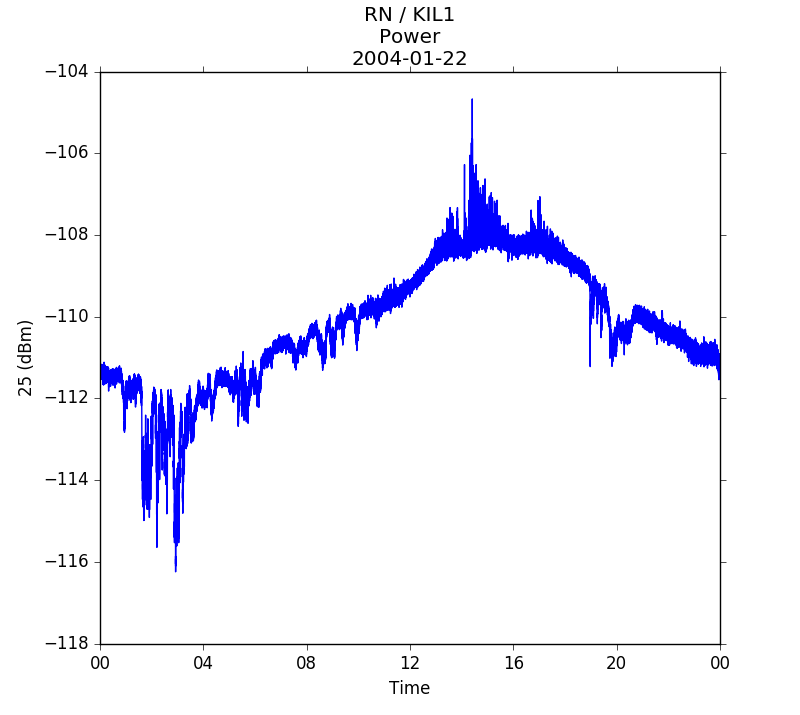
\includegraphics[width=9cm]{images/figure_1.png}

Hints on how to use functions such as {\it ap.load\_data} can be seen by appending a question mark to the function name.

\begin{lstlisting}[style=pythonstyle]
ap.load_data?

Definition:  ap.load_data(project, site, data_type, start_time, end_time, archive=None, channels=None, path=None, load_function=None, raise_all=False, cadence=None, aggregate=None, filter_function=None)
\end{lstlisting}

Each riometer has a site name (in this case 'KIL1'), and belongs to a particular project. 'RN' stands for the Riometer Network project. The archive name 'local archive' could be changed to 'remote archive' in order to load this example data from www.riometer.net. Sites, projects and archives are defined in the datasets module ({\it auroraplot.datasets.riometernet}).

Note that the channels are specified as a list of strings. When dealing with riometer data, channels (beams) are usually numbered from 1, but magnetometer channels may be named 'X', 'Y', and 'Z', or 'H', 'D', and 'Z'.


\subsubsection{Example 2: Making Quiet Day Curves}

To make a quiet day curve, it is necessary to load more than one day of data. Usually 14 days will suffice. By default, the valid period for a QDC will be 14 days long.
Auroraplot has functions in the ap.dt64tools package that can be used to find the standard boundaries for the QDCs: {\it ap.dt64tools.floor, and ap.dt64tools.ceil}. If the period is a multiple of one week, the boundary will start on a Monday.

\begin{lstlisting}[style=pythonstyle]
t = np.datetime64('2004-01-22T00:00:00')
st = ap.dt64tools.floor(t, np.timedelta64(14,'D'))
et = ap.dt64tools.ceil(t, np.timedelta64(14,'D'))
rd = ap.load_data('RN','KIL1','RioPower',st,et,'local archive',channels=['25'])
\end{lstlisting}

Here {\it st} holds the datetime64 value of '2004-01-12T00:00:00', and {\it et} is '2004-01-26T00:00:00'.

The QDC is made from the power data by calling make\_qdc().

\begin{lstlisting}[style=pythonstyle]
qdc = rd.make_qdc()
qdc.plot(channels=['25'])
\end{lstlisting}

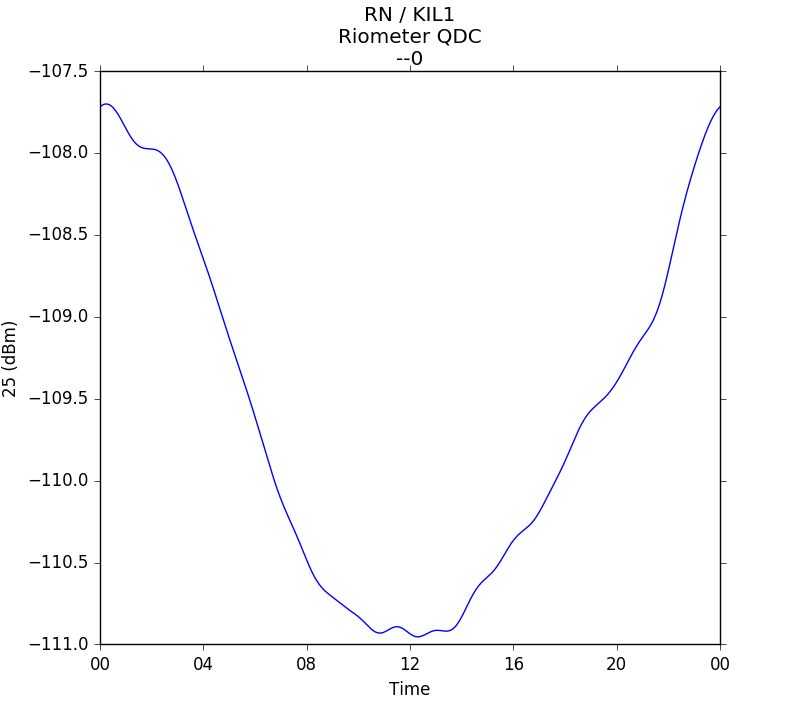
\includegraphics[width=9cm]{images/figure_2.png}


Calling make\_qdc() will create QDCs for all channels of the riometer (according to the metadata in auroraplot.datasets). But since {\it rd} only contains data for channel '25', calling {\it qdc.plot()}, without the {\it channels} argument will make a large number of mostly empty plots.

If the computer has sufficient RAM ($\ge 12$ GB recommended) data from all channels can be loaded at once. It is also advantageous to integrate the riometer to lower resolutions before creating the quiet day curve.

\begin{lstlisting}[style=pythonstyle]
rd = ap.load_data('RN','KIL1','RioPower',st,et,'local archive')
rd.set_cadence(np.timedelta64(10,'s'), inplace=True)
qdc = rd.make_qdc()
qdc.plot(channels=['24','25','31','32'])
\end{lstlisting}

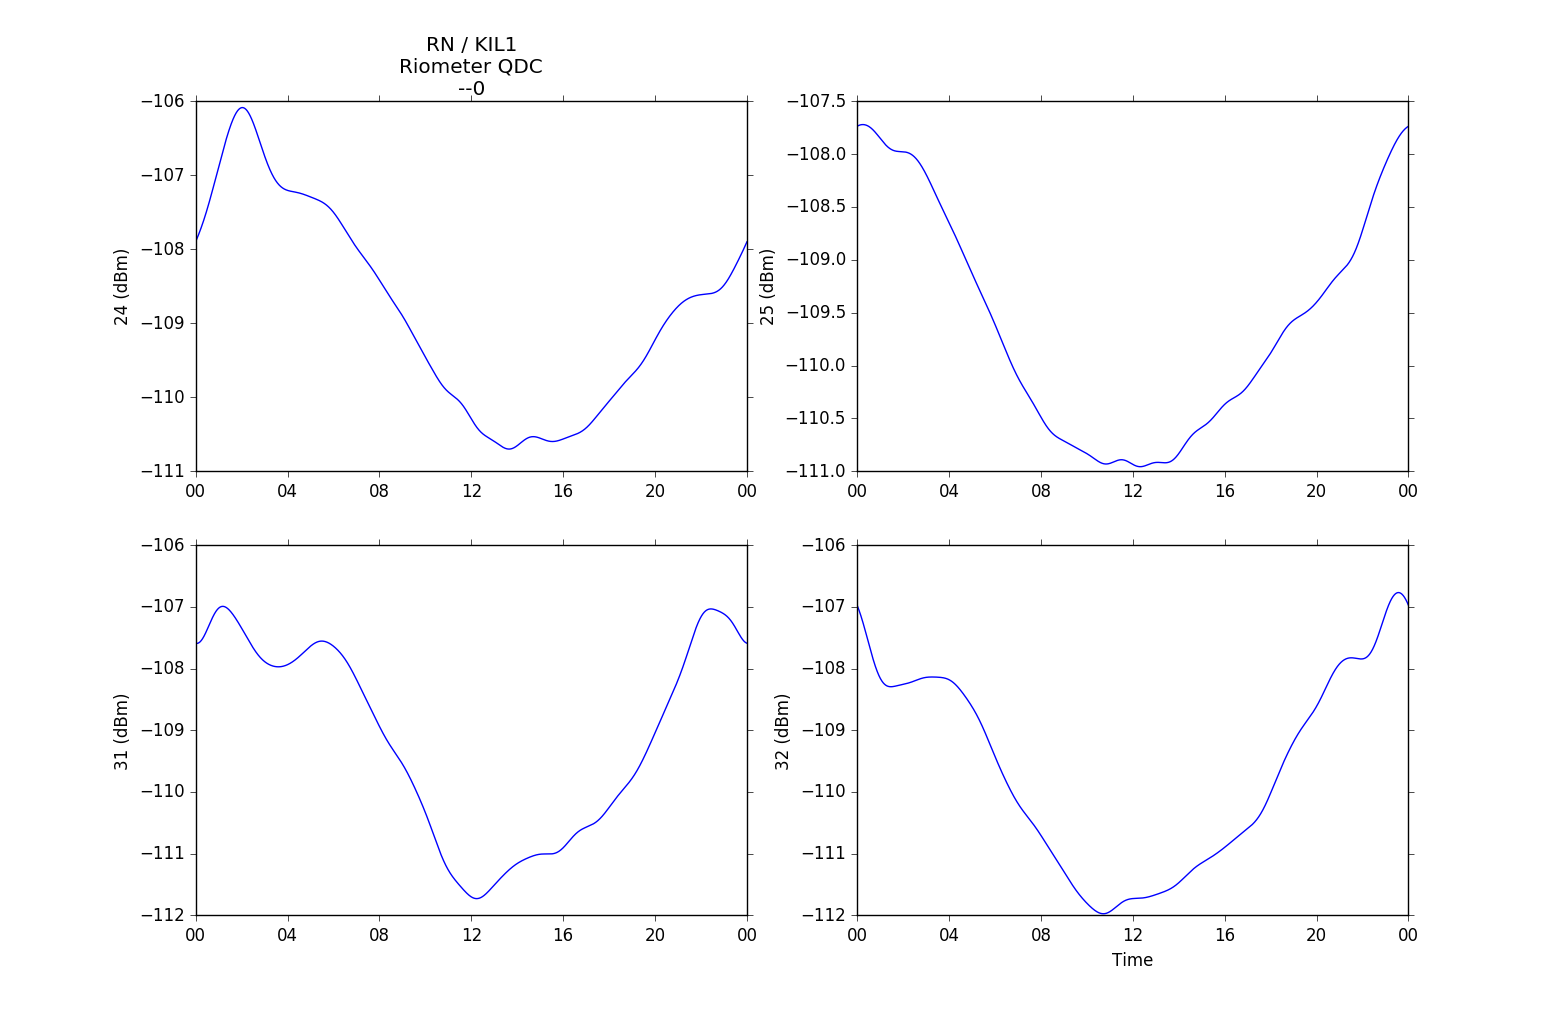
\includegraphics[width=12cm]{images/figure_3.png}


\noindent The argument inplace=True tells the set\_cadence function to overwrite {\it rd} instead of returning a copy of it with the new cadence (sampling interval).

The QDC can be saved for later use.

\begin{lstlisting}[style=pythonstyle]
qdc.save(archive='local archive', time=t)
\end{lstlisting}

\noindent where {\it time} is any numpy.datetime64 within the QDC's valid period. This will save the QDC data to /data/qdc/kil1/2004/kil1\_qdc\_20040112.txt.
The QDC can be reloaded by specifying the project, site, and a time within its valid period.
\begin{lstlisting}[style=pythonstyle]
qdc = ap.riodata.load_qdc('RN', 'KIL1', t, archive='local archive')
\end{lstlisting}

We can look again at the data from 22 January 2004, and this time plot it alongside the QDC.

\begin{lstlisting}[style=pythonstyle]
st = np.datetime64('2004-01-22T00:00:00')
et = st + np.timedelta64(1,'D')
rd = ap.load_data('RN','KIL1','RioPower',st,et,'local archive',channels=['25'])
rd.plot_with_qdc(qdc)
\end{lstlisting}

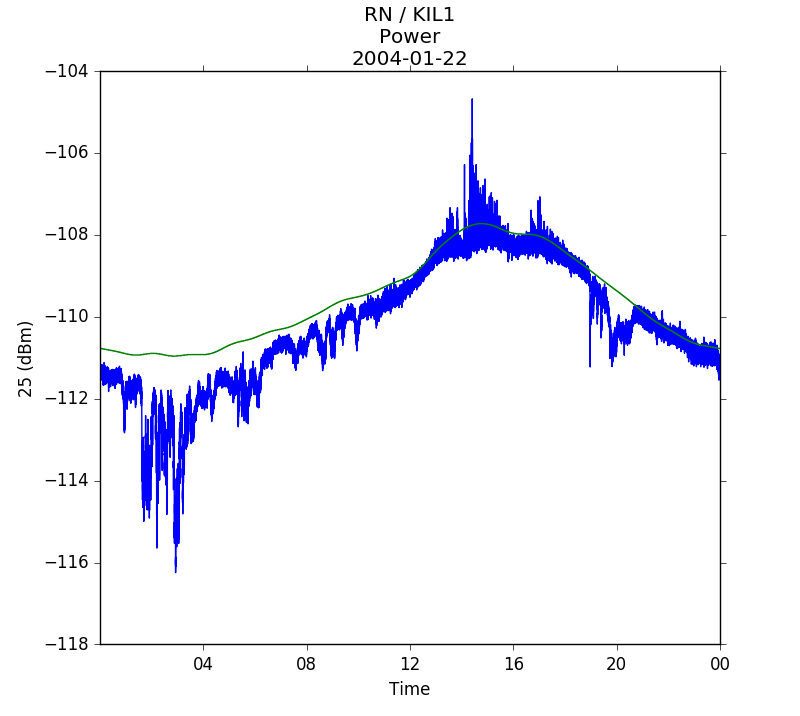
\includegraphics[width=9cm]{images/figure_4.png}


\noindent Alternatively, we can plot the ionospheric absorption (ie the quiet day curve minus the riometer received power).
\begin{lstlisting}[style=pythonstyle]
ab = rd.apply_qdc(qdc)
ab.plot()
\end{lstlisting}

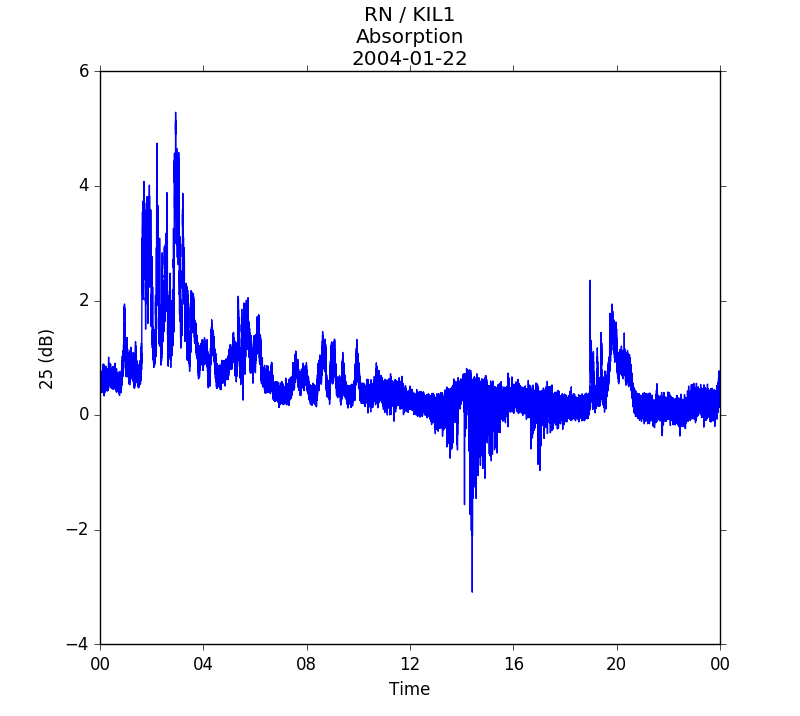
\includegraphics[width=9cm]{images/figure_5.png}

\subsubsection{Example 3: Integration of data and further processing}

In this example, we calculate the ionospheric absorption for the 21st, 22nd and 23rd of January, beams 25 and 26. Then integrate the data to 6-hour resolution, plot it, and extract the data for beam 25 for further processing in external functions. We will use the QDC saved in the previous example.

\begin{lstlisting}[style=pythonstyle]
st = np.datetime64('2004-01-21T00:00:00')
et = st + np.timedelta64(3,'D')
rd = ap.load_data('RN','KIL1','RioPower',st,et,'local archive',channels=['25','26'])
qdc = ap.riodata.load_qdc('RN', 'KIL1', st, archive='local archive')
ad = rd.apply_qdc(qdc)
ad6hr = ad.set_cadence(np.timedelta64(6,'h'))
ad6hr.plot(step_plot=True)
\end{lstlisting}

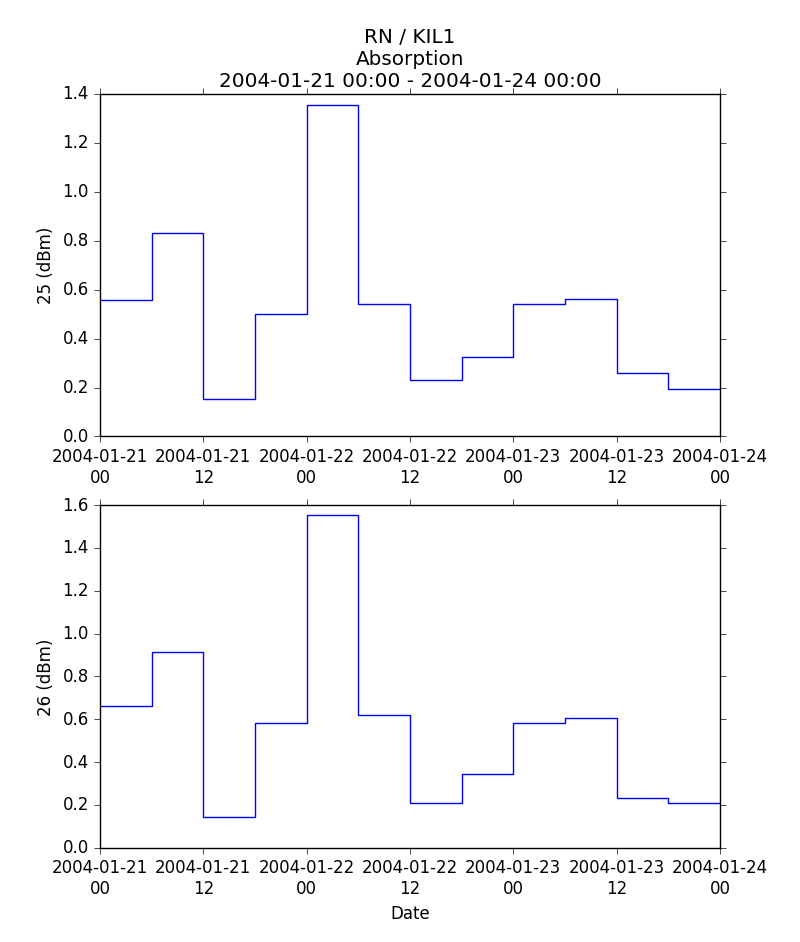
\includegraphics[width=9cm]{images/figure_6.png}

To extract beam 25 data, and find the central time of each sample.

\begin{lstlisting}[style=pythonstyle]
b25_index = ad6hr.get_channel_index(['25'])
b25_absorption_data = ad6hr.data[b25_index]
sample_central_time = ap.dt64tools.mean(ad6hr.sample_start_time,ad6hr.sample_end_time) 
\end{lstlisting}


\section{The Quick-Look Data Viewer}



\end{document}

